\chapter{Digitalizing the Cube}
\myTop{In order to implement solving algorithms on a Rubik's Cube the cube itself must first be digitalized and a visual interface must be created in order to see the result of an algorithm. In this chapter that process is described.}
A \rubik{} is a rather simple three-dimensional structure, but implementing this structure into a computer system and getting it depicted on a two-dimensional screen is not a simple task.
The \rubik{} is build up by 26 moving \cpiece{}s held together by each other.  This type of structure is not straight forward to implement into a computer, so a way to handle these \cpiece{}s is needed.

%If the \rubik{} is depicted in the computer in a two-dimensional space, its depiction will be far from the original \rubik{} structure.
A simple way to handle the \rubik{} in the program is a two-dimensional depiction and  just simply move the \facelet{}s around.
The analogue to this on a real \rubik{} would be to take the colored stickers off and move them to their new position rather than actually move the \cubie{}s when twisting the \rubik{}.
This approach would be far from reality and would make the implementation of solving algorithms, such as Kociemba's optimal solver and the beginner's algorithm more complicated, since they need to know the position of the \cpiece{}s, and not just the \facelet{}s in order to determine the next step.

A more object-oriented approach than to move the sticker would give a more useful structure for solving the problem.
If we divided the \rubik{} into its sub structures it would consist of six faces each with nine shared \cubie{}s.
%Dividing the \rubik{} into its sub structures. 
%The cube consist of the 6 faces each with 9 shared \cpiece{}. 
A face also consists of nine \cubicle{}s which act as placeholders for the \cpiece{}s. 
There are three types of \cpiece{}s and \cubicle{}s: corners, edges, and centers. 
The center \cpiece{}s will never move and therefore there is no reason to define a \cubicle{} and a \cpiece{} for those. Instead the center piece of a face is granted a colored \facelet{}, which defines the color of the face in the completed state of the \rubik{}.
\begin{figure}[h]
	\centering
		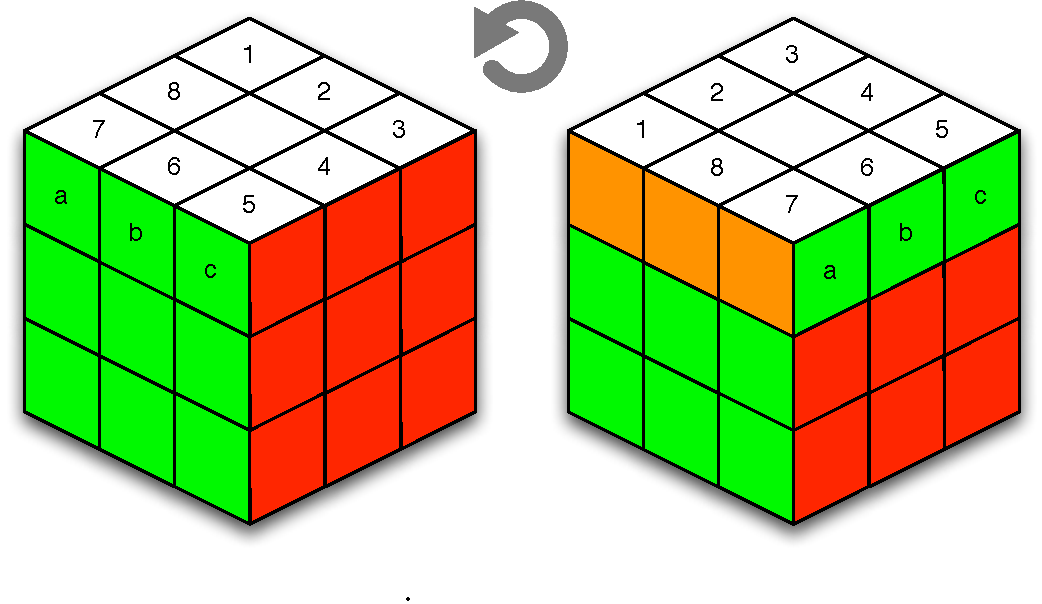
\includegraphics[scale=0.6]{input/pics/twistOfUpFace}
	\caption{\myCaption{A twist of a face will not only inflict the twisted face but also its adjacent faces. }}
	\label{fig:twistOfUpFace}
\end{figure}
This structure allows for the same \cubicle{} to be in several faces -- two faces for edges and three for corners. 
In this structure moving a \face{} will move the \cpiece{}s from one \cubicle{} to another. See figure \ref{fig:twistOfUpFace}. By performing a \twist{} the \face{}s adjacent to the twisted \face{} are also affected. 
For example when \twist{}ing the up face of a \rubik{} the \cubie{}s adjacent to the up face in R, L, B, and F faces will be permuted.

However the problem of this structure is that it requires variables to determine how the \cubie{}s are oriented. 
How this is done is described in the section \ref{sec:orientation}.

	\section{Orientation}
\label{sec:orientation}

\begin{figure}[h]
	\centering
		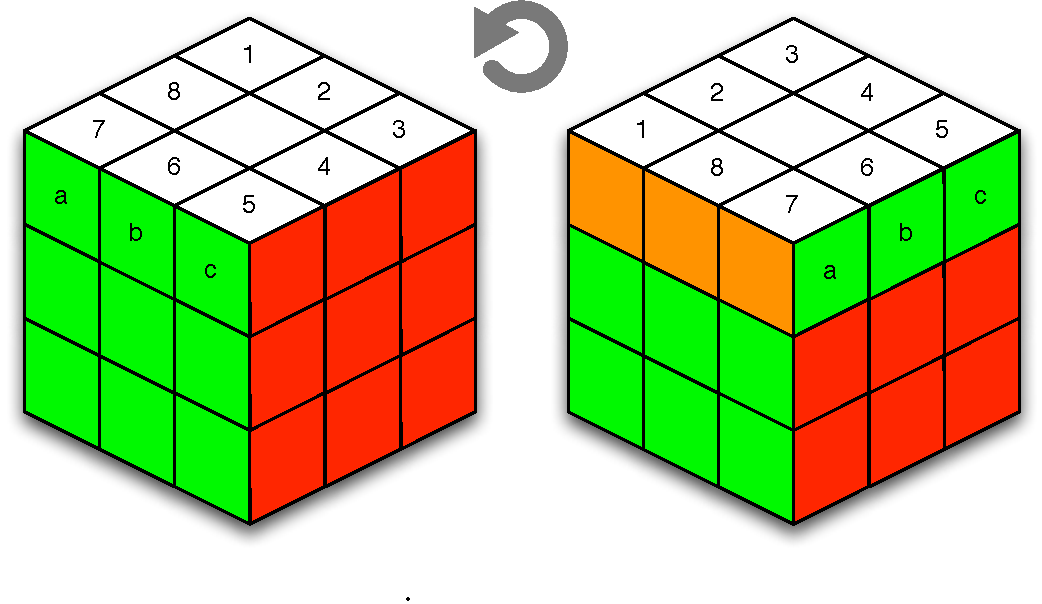
\includegraphics[scale=0.5]{input/pics/twistOfUpFace}
	\caption{\myCaption{A twist of a face will not only inflict the twisted face but also its adjacent faces. }}
	\label{fig:twistOfUpFace}
\end{figure}

In this structure moving a \face{} will move the \cpiece{}s from one \cubicle{} to another. See figure \ref{fig:twistOfUpFace}. By performing a \twist{} the \face{}s adjacent to the twisted \face{} are also affected. 
For example when \twist{}ing the up face of a \rubik{} the \cubie{}s adjacent to the up face in R, L, B, and F faces will be permuted.

However the problem of this structure is that it requires variables to determine how the \cubie{}s are oriented. 
How this is done is described in section \ref{sec:orientation}.
In order to draw a \rubik{} on the screen there are two things which are needed; the position of each \cubie{} and the orientation of each \cubie{}. This section will deal with the orientation of a \cubie{}.

The way to define an edge \cubie{} differs from the way to define a corner \cubie{}, which is why these to are dealt with separately.

In order to define the orientation of a \cubie{} it is needed to define different types of \face{}s, namely three types; primary, secondary, and tertiary. On a \rubik{} there is two \face{}s of each type. Each face of the same type is placed opposite to the other of the type. e.g. the white and yellow \face{}s could be primary because they are opposite to each other, blue and green could then be secondary, and red and orange would then be tertiary. See figure \ref{fig:cubeFaces} for an illustration of this example.

\begin{figure}[!hbt]
	\centering
		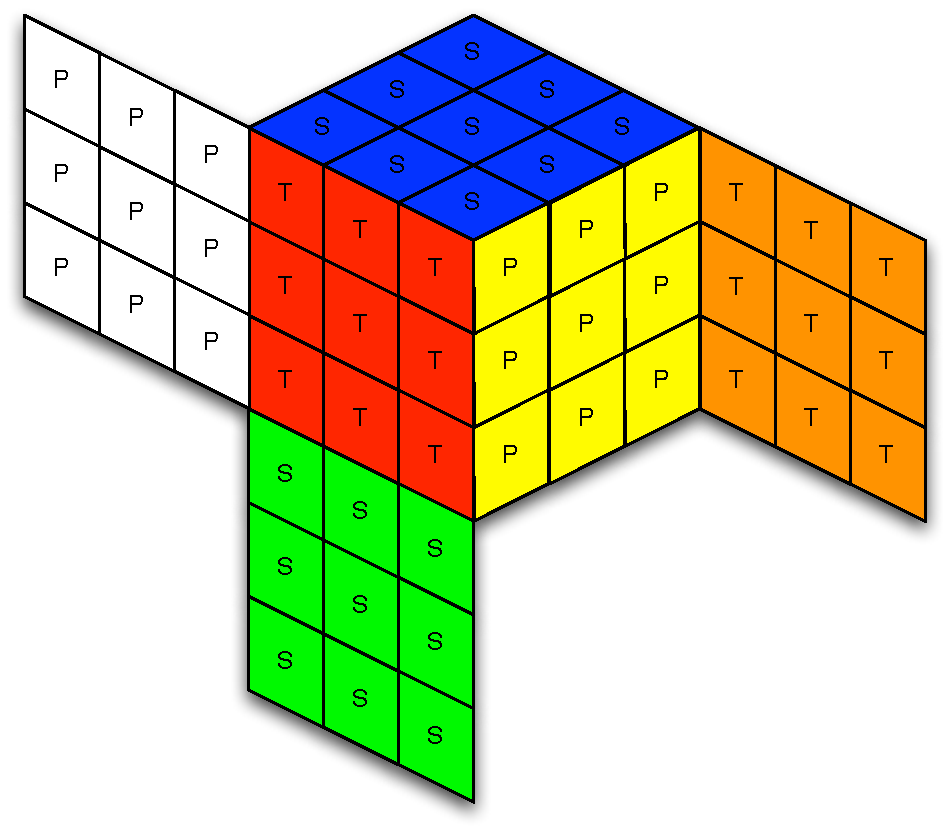
\includegraphics[width = 0.5\textwidth]{input/pics/cubeFaces}
	\caption{\myCaption{In this figure the two primary faces are labeled ``P'', the secondary faces ``S'', and the tertiary faces ``T''.}}
	\label{fig:cubeFaces}
\end{figure}


\subsection{Corner Cubie}
A corner \cubie{} in a given \cubicle{} can ``sit'' in this \cubicle{} in one of three ways. See figure \ref{fig:orientation} for the three different orientations of the white/blue/red corner \cubie{}.
Since each corner \cubie{} has one of each \facelet{} type -- one primary, one secondary, and one tertiary -- the orientation can be defined from where one of these \facelet{}s are positioned.
These different orientations can thereby be defined with an integer between 0 and 2.
0 if the primary \facelet{} of the \cubie{} is on the primary \face{}, 1 if the primary \facelet{} is on the secondary \face{}, and 2 if the primary \facelet{} is on the tertiary \face{}.

\begin{figure}[htb]
	\centering
		\subfloat[\myCaption{The white/blue/red corner is correctly oriented, which gives it the orientation value 0.}]{\label{fig:orientation:orientation0}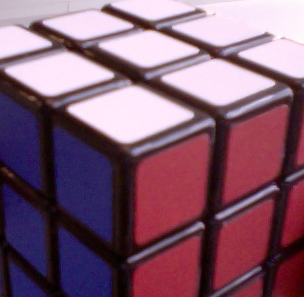
\includegraphics[width=0.28\textwidth]{input/pics/orientation0}}
		\hspace{0.02\textwidth}
		\subfloat[\myCaption{The white/blue/red corner is incorrectly oriented, the orientation value of this is 1 since the primary color is on a secondary face.}]{\label{fig:orientation:orientation1}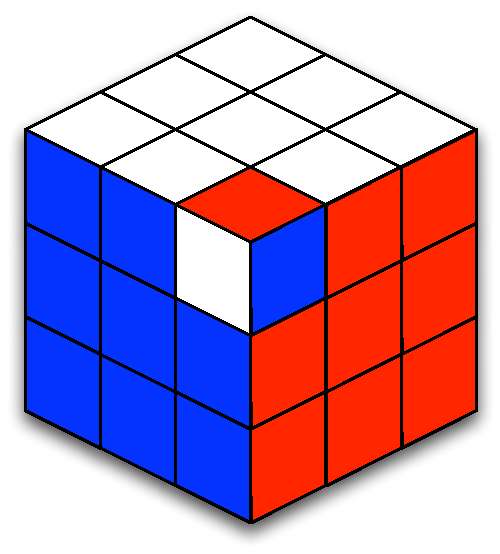
\includegraphics[width=0.28\textwidth]{input/pics/orientation1}}
		\hspace{0.02\textwidth}
		\subfloat[\myCaption{The white/blue/red corner is incorrectly oriented, the orientation value of this is 2 since the primary color is on a tertiary face.}]{\label{fig:orientation:orientation2}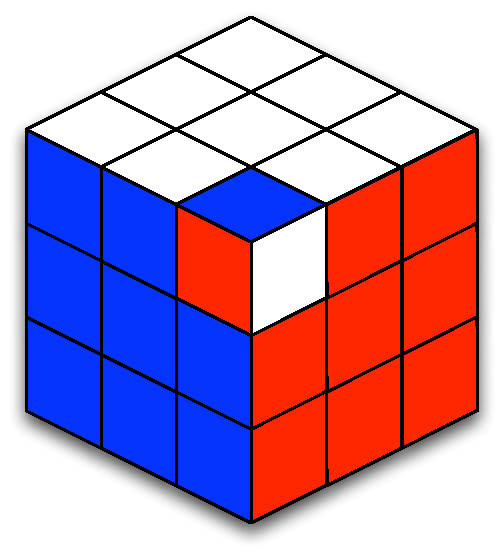
\includegraphics[width=0.28\textwidth]{input/pics/orientation2}}
		\caption{\myCaption{The three different orientation which the white/blue/red cubie can have. In these figures the white and yellow faces are primary, the blue and green are secondary, and red and orange are tertiary.}}
		\label{fig:orientation}
\end{figure}

In order to make it easier to draw the \rubik{} a secondary orientation is added. This orientation is defined from which \face{} the secondary \facelet{} is on.
This orientation is also defined from an integer between 0 and 2.
0 if the secondary \facelet{} of the \cubie{} is on the primary \face{}, 1 if the secondary \facelet{} is on the secondary \face{}, and 2 if the secondary \facelet{} is on the tertiary \face{}.
Note that a correctly oriented \cubie{} will have primary orientation 0 and secondary orientation 1.
It will also be easy to define a tertiary orientation of a \cubie{} by where the tertiary \facelet{} is positioned, but this will be redundant since this integer will always have the remaining value, e.g. the primary orientation is 0, the secondary orientation is 1, then the tertiary orientation must be 2.
See figure \ref{fig:orientationFlow} for a flowchart on how to find the primary and/or the secondary orientation of a corner \cubie{}.

\subsection{Edge Cubie}
The orientation of an edge \cubie{} can be defined with a boolean value; either it is correctly oriented or it is not.
This is easiest to see when the \cubie{} is in the right position.
If the white/blue edge \cubie{} is in its correct \cubicle{} then it is correctly oriented if the white \facelet{} is on the white \face{} and the blue \facelet{} is on the blue \face{}.
The \cubie{} is wrongly oriented if the blue \facelet{} is on the white \face{} and the white \facelet{} is on the blue \face{}.

This raises the question: What is the orientation of a \cubie{} which is not in its correct \cubicle{}?
This was not too difficult with corner \cubie{}s because they always had a \facelet{} of each type, which an edge \cubie{} does not. An edge \cubie{} can be one of the following combinations of \facelet{} types: Primary/secondary, primary/tertiary, or secondary/tertiary. With this knowledge it is possible to simply look at the ``highest'' \facelet{}, meaning the \facelet{} with the highest rank.
The rank refers to the type of \facelet{}, where primary is the highest, secondary the second highest rank, and tertiary the lowest.
Then define the orientation as the following: If the highest \facelet{} of a \cubie{} is on the highest \face{}, then the \cubie{} is correctly oriented.
In order to stay in connection with corner \cubie{} the correct orientation of a \cubie{} is given the number 0 and the incorrect orientation the number 1.
Note that this is opposite to what is usually done in programming where 1 is true and 0 is false \cite{boolean2}.
See the flowchart in figure \ref{fig:orientationFlow}.

\begin{figure}[hbp]
	\centering
		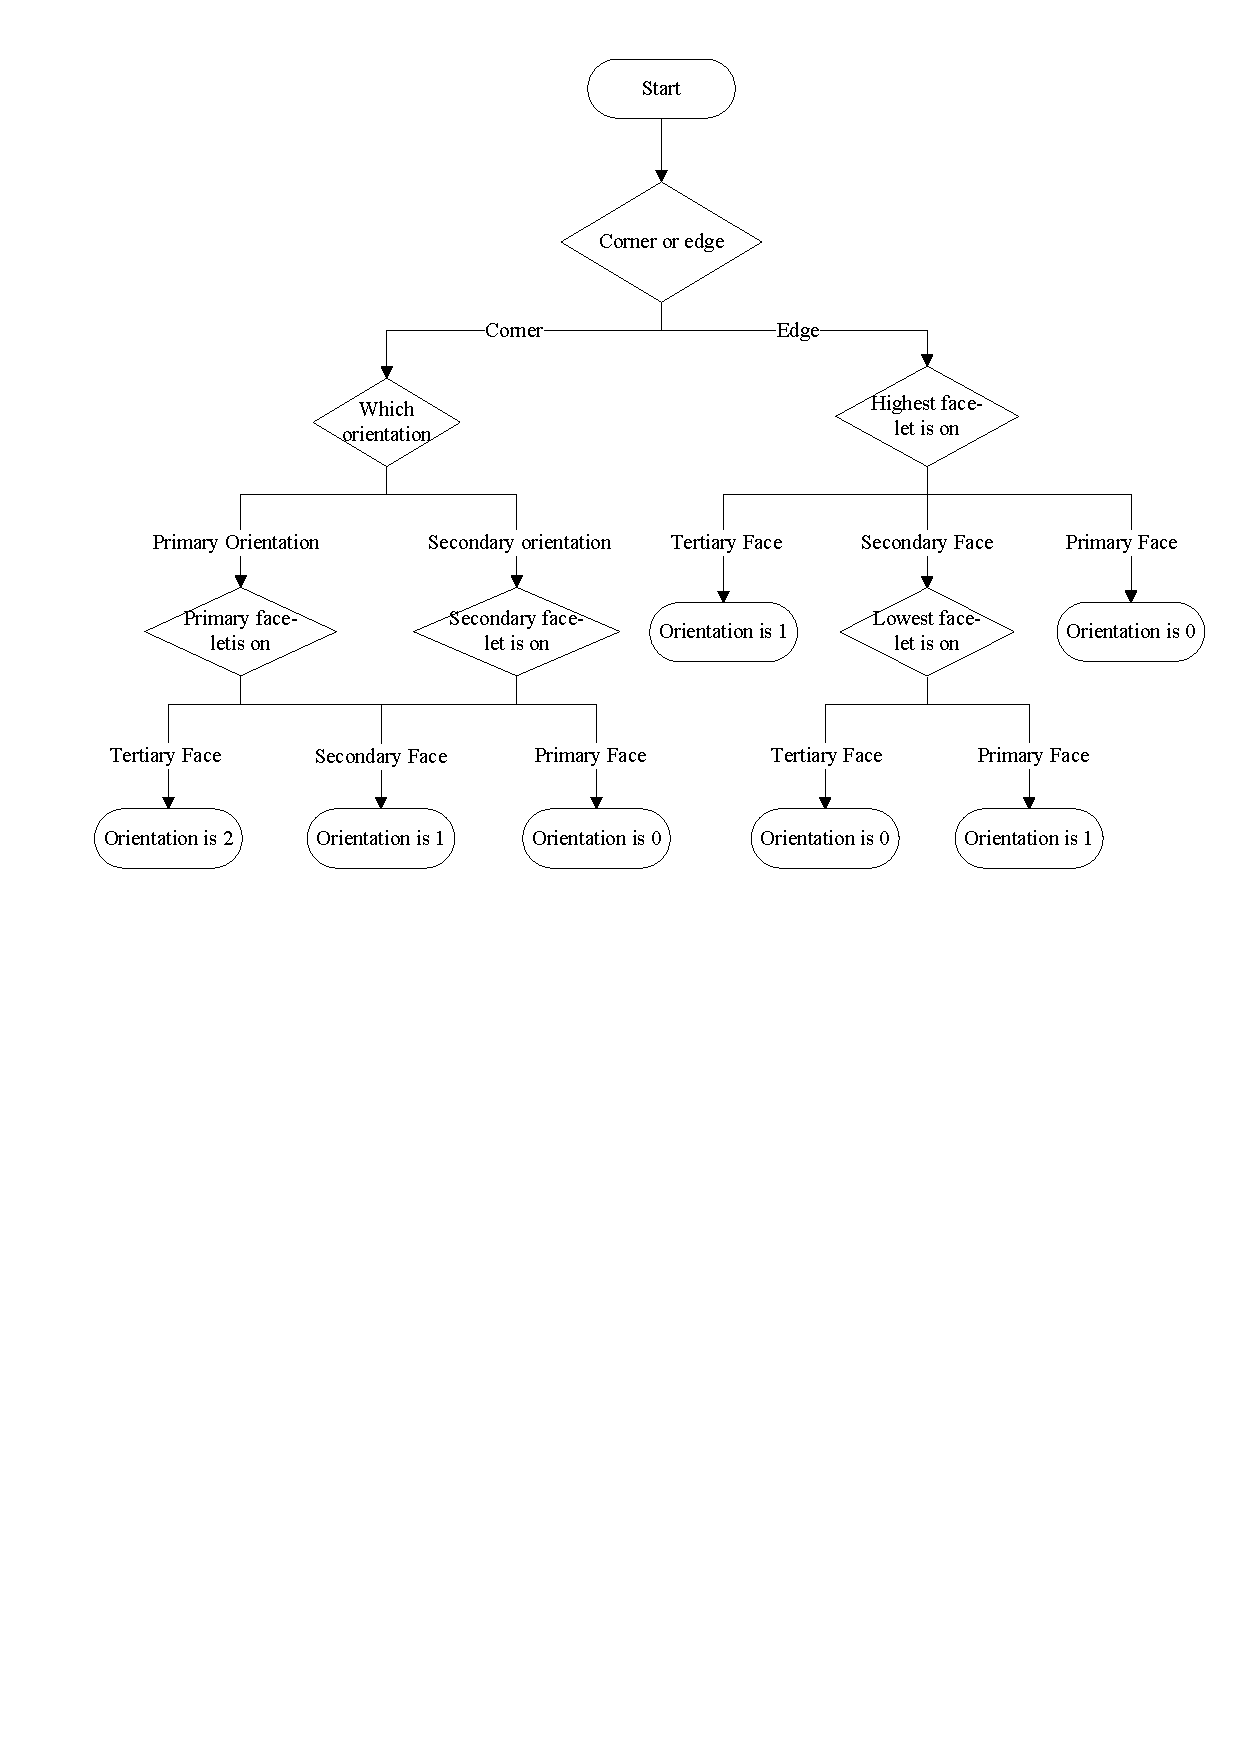
\includegraphics[width = \textwidth, trim = 10mm 150mm 0mm 10mm, clip]{input/pics/orientationFlow}
	\caption{\myCaption{Follow this flowchart to get the orientation of a cubie.}}
	\label{fig:orientationFlow}
\end{figure}

	\section{The cube structure}
%In this section the different classes of the \rubik{} and their interaction with each other will be determined.
In this implementation we used a more object orientated approach to the problem.
The \rubik{} is divided into its sub structures which consist of six faces each with nine shared \cubicle{}s each containing a \cubie{}. The \cubie{}s either consist of one, two or three facelets. On figure \ref{fig:cubeClassDiagram} the cube class diagram is shown and a detailed description of the classes will explained in the following subsections.
%The cube consist of the 6 faces each with 9 shared \cpiece{}. 

\begin{figure}[htbp]
	\centering
		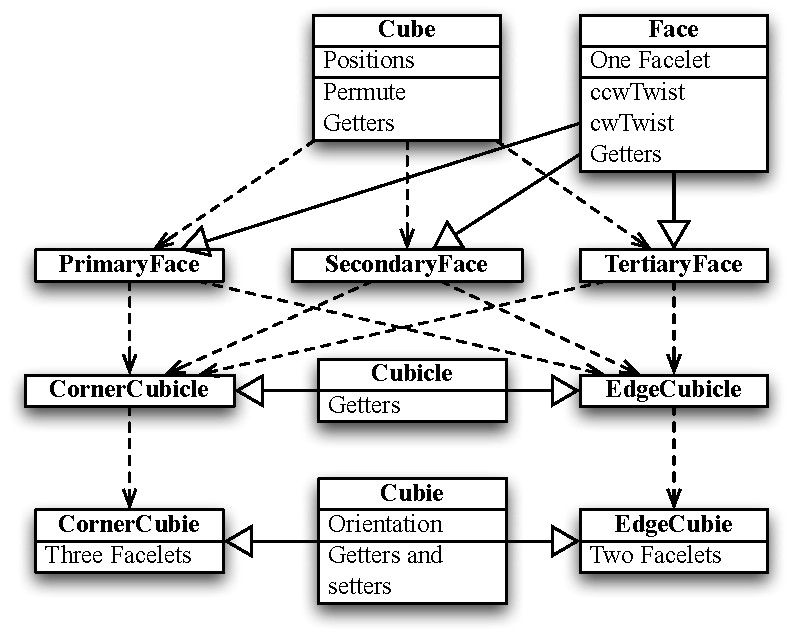
\includegraphics[scale=0.75]{input/pics/cubeClassDiagram.pdf}
	\caption{Class diagram of the cube with properties and methods}
	\label{fig:cubeClassDiagram}
\end{figure}


There are three types of \cpiece{}s and \cubicle{}s: corners, edges, and centers. 

\subsection{The Cube}
The cube class creates the 20 \cubicle{}s in which the \cpiece{}s can be positioned. Furthermore the cube class creates the \face{}s and \cubie{}s. Eventhough the cube class initialize all objects this is not drawn on the class diagram (figure \ref{fig:cubeClassDiagram}) because they are not used this way. The cube class also gives each \cpiece{} its \facelet{}s. The \cubicle{}s are then put into a \face{} by its constructor. The cube class creates six \face{}s -- two primary, two secondary and two tertiary faces. Each type of \face{}s are placed opposite to each other. e.g. the up and down faces are both primary. The cube has a static method, \vr{permute}, it has two arguments, a cube and a sequence of \twist{}. The \twist{}s are applied to the cube.

\subsection{The Face}
A face consists of nine \cubicle{}s which act as placeholders for the \cpiece{}s. The center \cpiece{}s will never move and therefore there is no reason to define a \cubicle{} and a \cpiece{} for those. Instead the center piece of a face is granted a colored \facelet{}, which defines the color of the face in the completed state of the \rubik{}.
The \face{} class constructor takes eight cubicles (four corners and four edges) and position them in a clockwise order. In addition the \face{} class implements two methods which twist the face clockwise or counterclockwise -- namely \textit{cwTwist} and \textit{ccwTwist} respectively.

There are three different types of \face{}s; primary \face{}s, secondary \face{}s, and tertiary \face{}s.
Each type has its own subclass, which inherits from the \face{} superclass.
The reason for the different classes is that there is a difference in how the orientation of the \cubie{}s changes depending on what type of \face{} being \twist{}ed.
%Orientation of \cubie{}s will be covered in ref\{orientation\}.

\subsection{The Cubicle}
%Måske noget om cubicle class, hvis der bliver lavet noget.
The \cubicle{} class is a superclass and there are two subclasses to this class corner- and edge \cubicle{}.
The corner and edge \cubicle{} classes each has one instance variable, namely the \cubie{} they hold. The \cpiece{} is set by the constructor of the \cubicle{} class.

\subsection{The Cubie}
The \cpiece{} class sets the orientation correctly by default, and it implements methods that return the orientation and \facelet{}s of the \cpiece{}. The corner and edge \cpiece{} classes implements two different methods which return the orientation of the \cpiece{}. The \cubie{} class is a superclass and there are two subclasses to this corner- and edge \cubie{}. The corner \cubie{} contains three facelets, where edge \cubie{} only contains two facelets.

\subsection{The Facelet}
%%The \facelet{} class is an enumeration that contains the colors of the \facelet{}s, it implements a \textit{toColor} method which define the color of each \facelet{}.
The \facelet{}s are defined in an enumeration which contains the colors of the \facelet{}s, it implements a \textit{toColor} method which define the actual color of each \facelet{}.